% ------------------------------------------------------------------------------
% TYPO3 CMS 7.2 - What's New (English Version)
%
% @author	Michael Schams <schams.net>
% @license	Creative Commons BY-NC-SA 3.0
% @link		http://typo3.org/download/release-notes/whats-new/
% @language	English
% ------------------------------------------------------------------------------
% LTXE-CHAPTER-UID:		93899f32-8efb477e-ed6973d2-b679bd8e
% LTXE-CHAPTER-NAME:	Backend User Interface
% ------------------------------------------------------------------------------

\section{Interfaz de Usuario de Backend}
\begin{frame}[fragile]
	\frametitle{Interfaz de Usuario de Backend}

	\begin{center}\huge{Capítulo 1:}\end{center}
	\begin{center}\huge{\color{typo3darkgrey}\textbf{Interfaz de Usuario de Backend}}\end{center}

\end{frame}

% ------------------------------------------------------------------------------
% LTXE-SLIDE-START
% LTXE-SLIDE-UID:		db1c6a07-dfec75a0-9a1fd5c0-171eb879
% LTXE-SLIDE-ORIGIN:	c151f95c-3fe3eb42-442ce244-5f987f80 English
% LTXE-SLIDE-TITLE:		Customized BE login form
% LTXE-SLIDE-REFERENCE:	unknown
% ------------------------------------------------------------------------------
\begin{frame}[fragile]
	\frametitle{Interfaz de Usuario de Backend}
	\framesubtitle{Formulario de ingreso personalizable}

	La extensión de sistema \texttt{backend} permite que los administradores 
	configuren una imagen de fondo personalizada, un logo y un color para la 
	pantalla de inicio del backend:

	\begin{figure}
		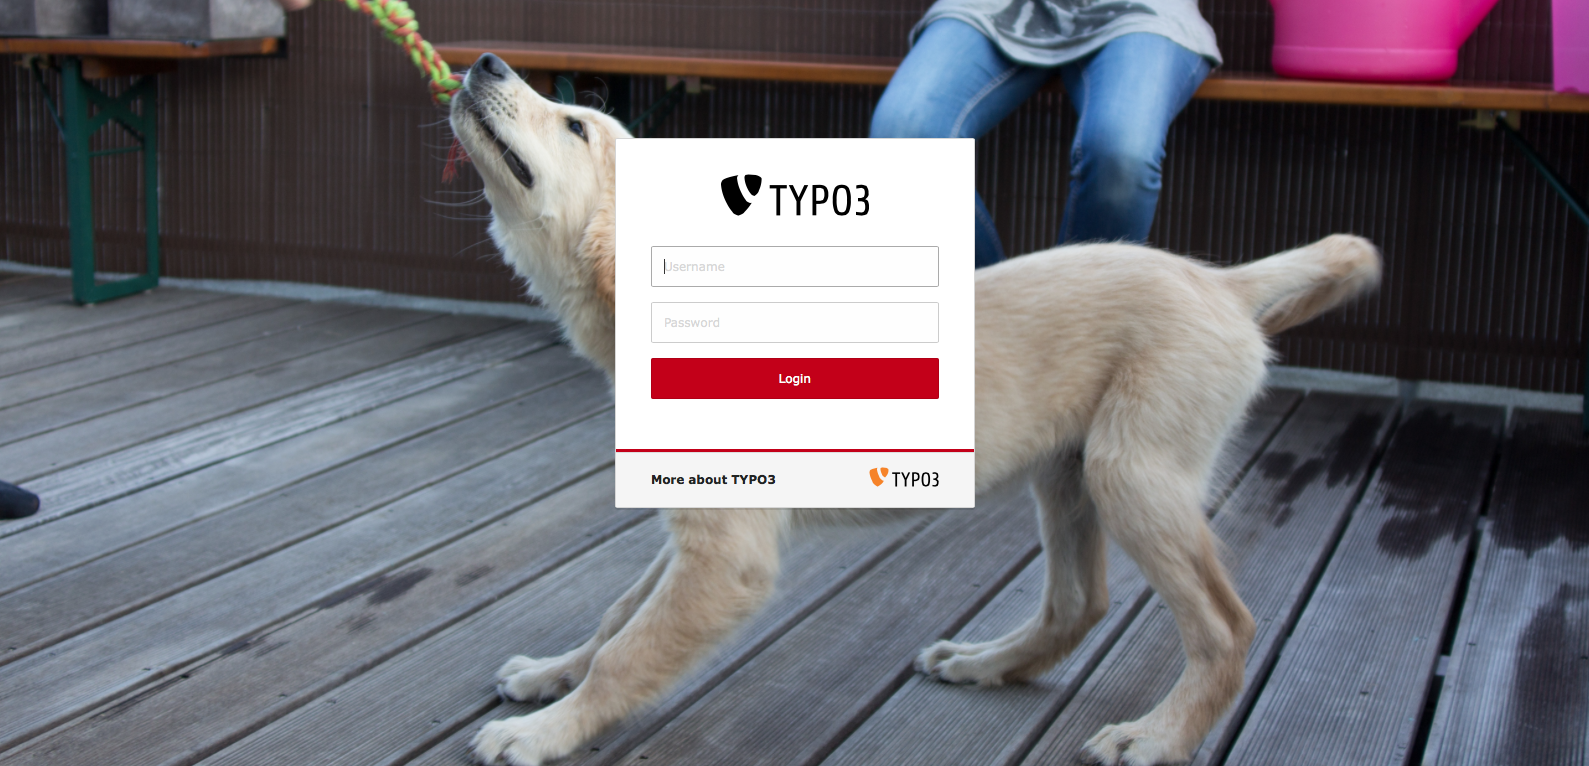
\includegraphics[width=0.75\linewidth]{BackendUserInterface/Login.png}
	\end{figure}

\end{frame}

% ------------------------------------------------------------------------------
% LTXE-SLIDE-START
% LTXE-SLIDE-UID:		4d438099-7d8897ac-52cb2117-195710c2
% LTXE-SLIDE-ORIGIN:	e2e353ae-3b2b5c00-0cd7c57d-d97d22c9 English
% LTXE-SLIDE-TITLE:		Add image cropping
% LTXE-SLIDE-REFERENCE:	Feature-65584-AddImageCropping.rst
% ------------------------------------------------------------------------------
\begin{frame}[fragile]
	\frametitle{Interfaz de Usuario de Backend}
	\framesubtitle{Manipulación de la Imagen: Recortar}

	Una función de manipulación de imagen permite que los editores ajusten las 
	imágenes en el backend. Esta característica debe ser explícitamente 
	activada para usuarios BE ("Exclude Fields"):

	\begin{figure}
		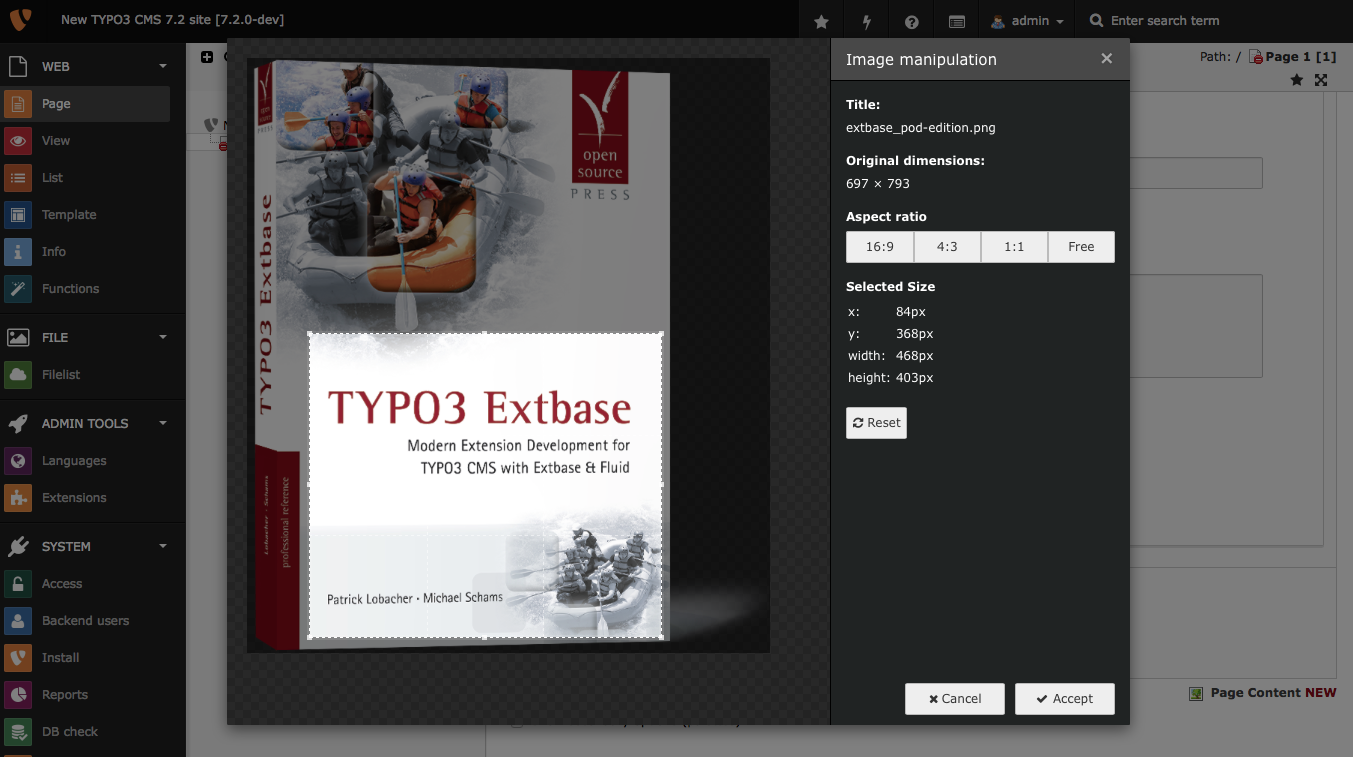
\includegraphics[width=0.7\linewidth]{BackendUserInterface/ImageCropping.png}
	\end{figure}

\end{frame}

% ------------------------------------------------------------------------------
% LTXE-SLIDE-START
% LTXE-SLIDE-UID:		dd1ce6d0-ec4b0af2-c1906135-c0739d02
% LTXE-SLIDE-ORIGIN:	301dfea9-d2debf3e-dcaa7bcd-205e5990 English
% LTXE-SLIDE-TITLE:		Add backend user groups to backend user module
% LTXE-SLIDE-REFERENCE:	Feature-64686-AddBackendUserGroupsToBackendUserModule.rst
% ------------------------------------------------------------------------------
\begin{frame}[fragile]
	\frametitle{Interfaz de Usuario de Backend}
	\framesubtitle{Grupos de Usuarios Backend}

	Los grupos de usuarios Backend pueden ser mantenidos en un sub-módulo del 
	módulo "Usuarios Backend":

	\begin{figure}
		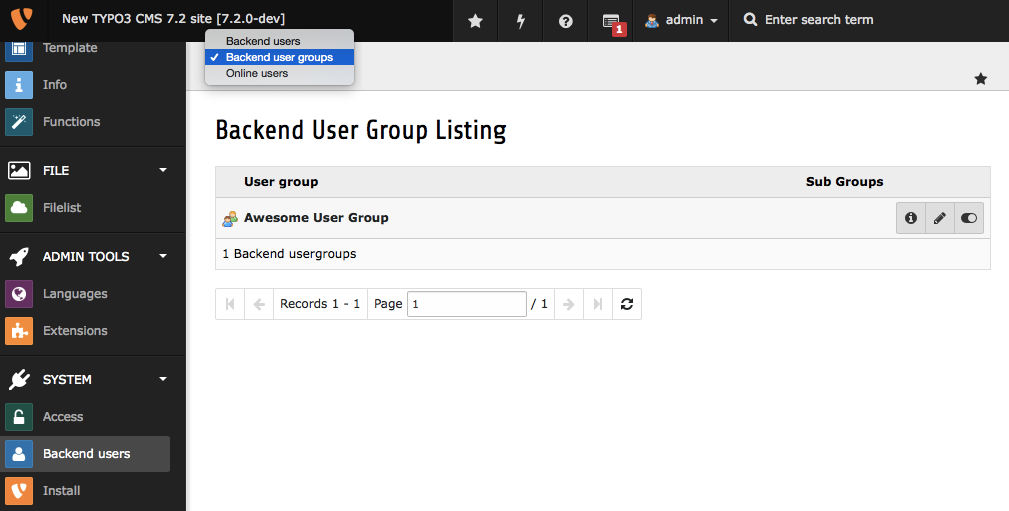
\includegraphics[width=0.70\linewidth]{BackendUserInterface/UserGroups.png}
	\end{figure}

\end{frame}

% ------------------------------------------------------------------------------
% LTXE-SLIDE-START
% LTXE-SLIDE-UID:		472ff3f4-96b8f544-186b749c-f67b7550
% LTXE-SLIDE-ORIGIN:	daa83c1e-08d2716b-de74cbda-42361551 English
% LTXE-SLIDE-TITLE:		Extension Manager: Disable automatic installation
% LTXE-SLIDE-REFERENCE:	Feature-50501-DisableAutomaticExtInstallation.rst
% ------------------------------------------------------------------------------
\begin{frame}[fragile]
	\frametitle{Interfaz de Usuario de Backend}
	\framesubtitle{Deshabilitar Instalación Automática de Extensiones}

	Los administradores pueden configurar el Administrador de Extensiones
	para que no se instalen extensiones descargadas de manera inmediata:

	\begin{figure}
		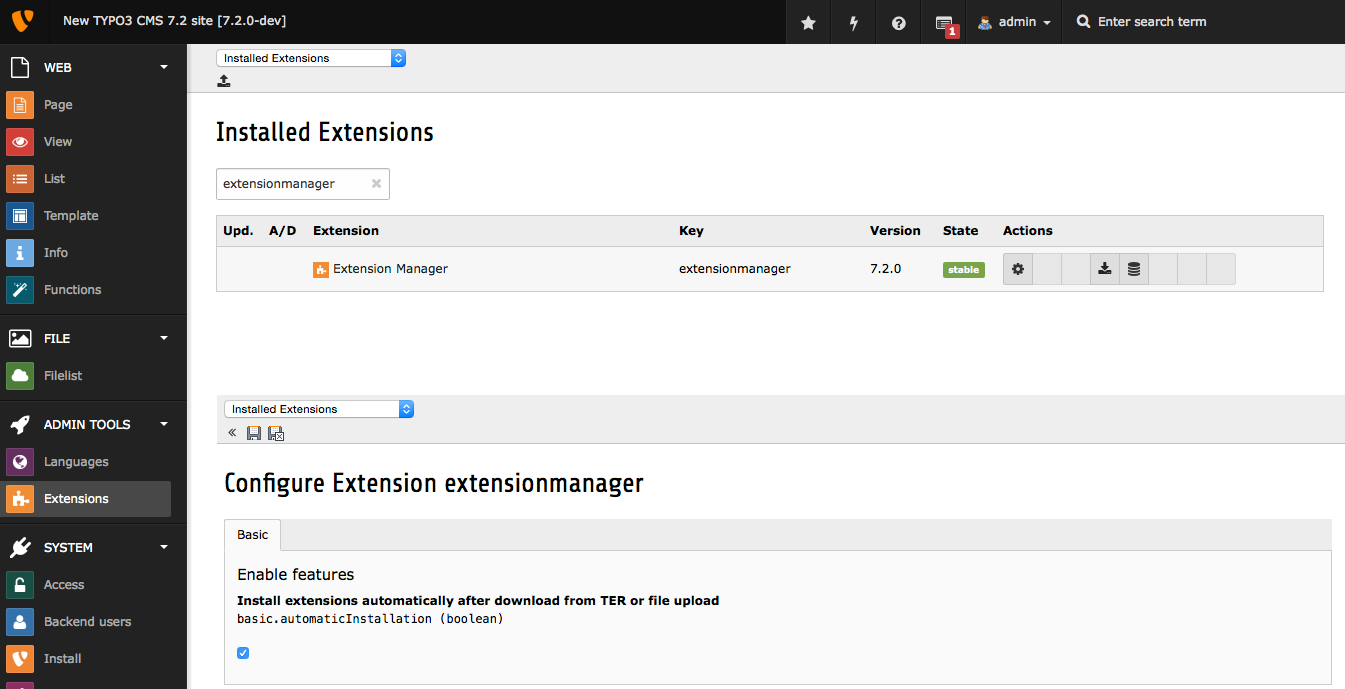
\includegraphics[width=0.70\linewidth]{BackendUserInterface/ExtManager.png}
	\end{figure}

\end{frame}

% ------------------------------------------------------------------------------
% LTXE-SLIDE-START
% LTXE-SLIDE-UID:		b1686769-60ab2306-0febd199-05f8394c
% LTXE-SLIDE-ORIGIN:	20769920-da9df227-c3b527b9-9a23bac1 English
% LTXE-SLIDE-TITLE:		Show remaining characters below text fields
% LTXE-SLIDE-REFERENCE:	Feature-66029-ShowRemainingCharactersBelowTextFields.rst
% ------------------------------------------------------------------------------
\begin{frame}[fragile]
	\frametitle{Interfaz de Usuario de Backend}
	\framesubtitle{Caracteres Restantes en campos de texto}

	El número de caracteres restantes es mostrado debajo del campo de ingreso de texto:

	\begin{figure}
		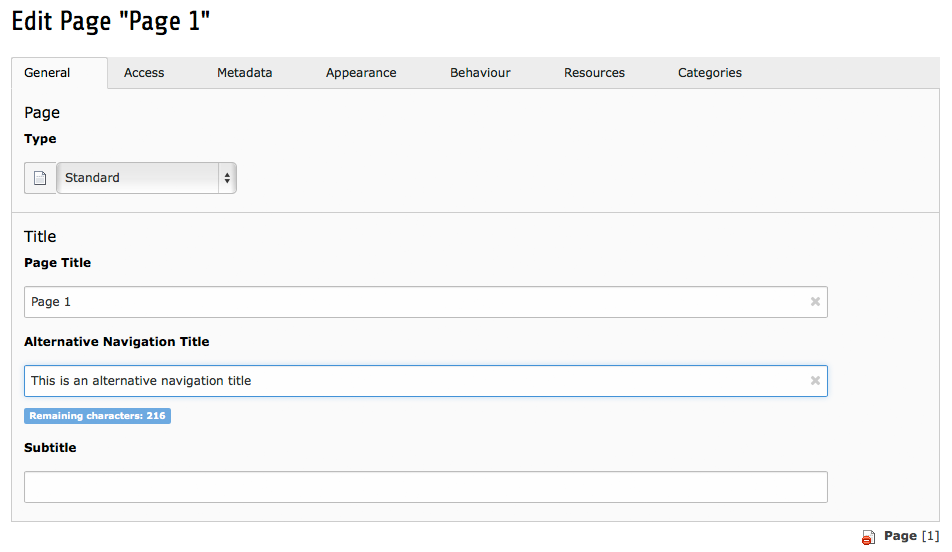
\includegraphics[width=0.70\linewidth]{BackendUserInterface/RemainingCharacters.png}
	\end{figure}

\end{frame}

% ------------------------------------------------------------------------------
% LTXE-SLIDE-START
% LTXE-SLIDE-UID:		31b0548f-81684a89-ac3eda19-efcf6660
% LTXE-SLIDE-ORIGIN:	ff760b86-9d6b1ecd-d0e98565-f23c51f0 English
% LTXE-SLIDE-TITLE:		Show confirm message on closing an editform with unsaved changes
% LTXE-SLIDE-REFERENCE:	Feature-65996-AddConfirmationOnCloseEditformWithUnsavedChanges.rst
% ------------------------------------------------------------------------------
\begin{frame}[fragile]
	\frametitle{Interfaz de Usuario de Backend}
	\framesubtitle{Confirmar Cambios no Guardados}

	Un nuevo cuadro de diálogo advierte a los editores de perder cambios no guardados:

	\begin{figure}
		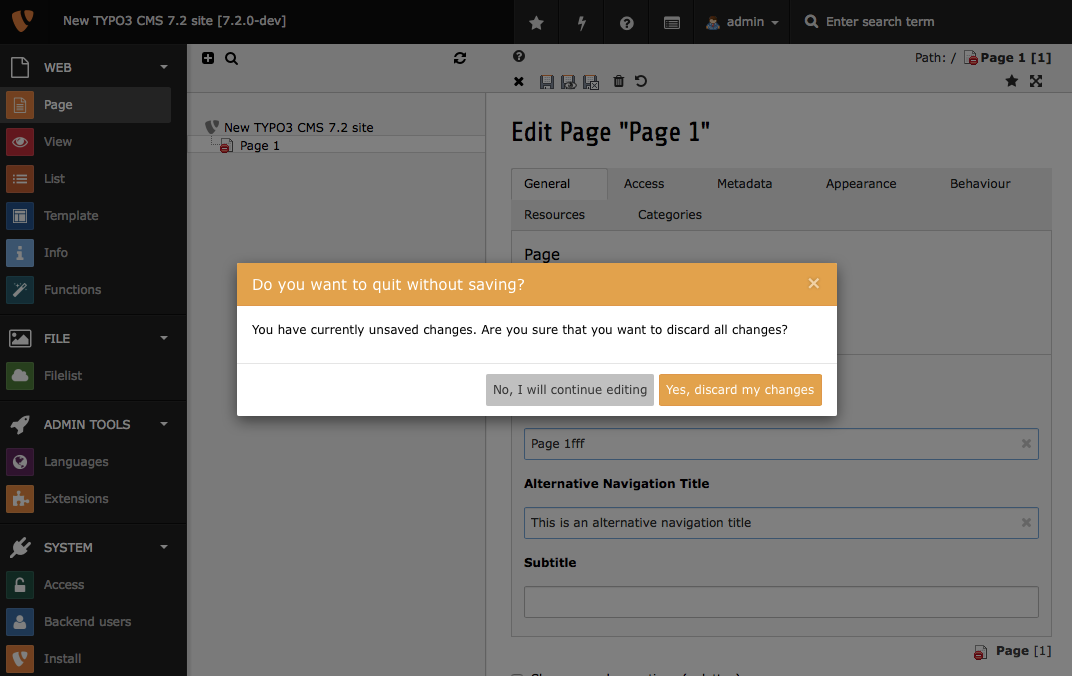
\includegraphics[width=0.65\linewidth]{BackendUserInterface/ClosingDialog.png}
	\end{figure}

\end{frame}

% ------------------------------------------------------------------------------
% LTXE-SLIDE-START
% LTXE-SLIDE-UID:		f750989a-12bf3271-dc23977d-429590f7
% LTXE-SLIDE-ORIGIN:	6ac9a35e-46541895-7509263e-28fb799f English
% LTXE-SLIDE-TITLE:		System Information Dropdown
% LTXE-SLIDE-REFERENCE:	Feature-65767-SystemInformationDropdown.rst
% ------------------------------------------------------------------------------
\begin{frame}[fragile]
	\frametitle{Interfaz de Usuario de Backend}
	\framesubtitle{Menú desplegable de Información del Sistema}

	Un menú desplegable muestra diversa información sobre el sistema donde TYPO3
	está instalado. Los datos de este cuadro pueden ser ampliados:\newline
	\small(ver el capítulo "Cambios en Profundidad" para más detalles)\normalsize

	\begin{figure}
		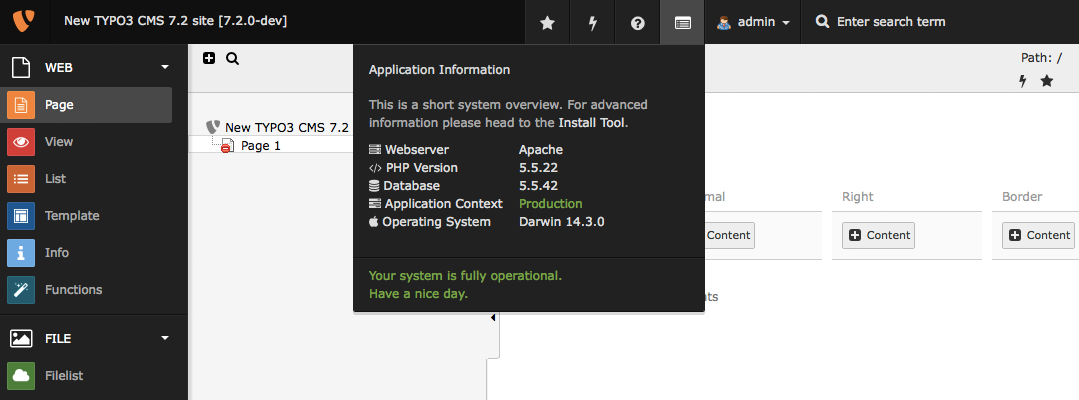
\includegraphics[width=0.85\linewidth]{BackendUserInterface/SystemInformation.png}
	\end{figure}

\end{frame}

% ------------------------------------------------------------------------------
% LTXE-SLIDE-START
% LTXE-SLIDE-UID:		a95bfc1f-922ed334-d3e8d5d1-05c2b961
% LTXE-SLIDE-ORIGIN:	79a2ee0c-3439d600-08990adb-6bed8c19 English
% LTXE-SLIDE-TITLE:		Ask for old password when changing
% LTXE-SLIDE-REFERENCE:	commit bf6f5226eb6cb441bb53657a88ef42f1cdb5155f
% ------------------------------------------------------------------------------
\begin{frame}[fragile]
	\frametitle{Interfaz de Usuario de Backend}
	\framesubtitle{Cambiar Contraseña}

	Los usuarios del backend deben proporcionar la contraseña actual con el fin de
	establecer una contraseña nueva:

	\begin{figure}
		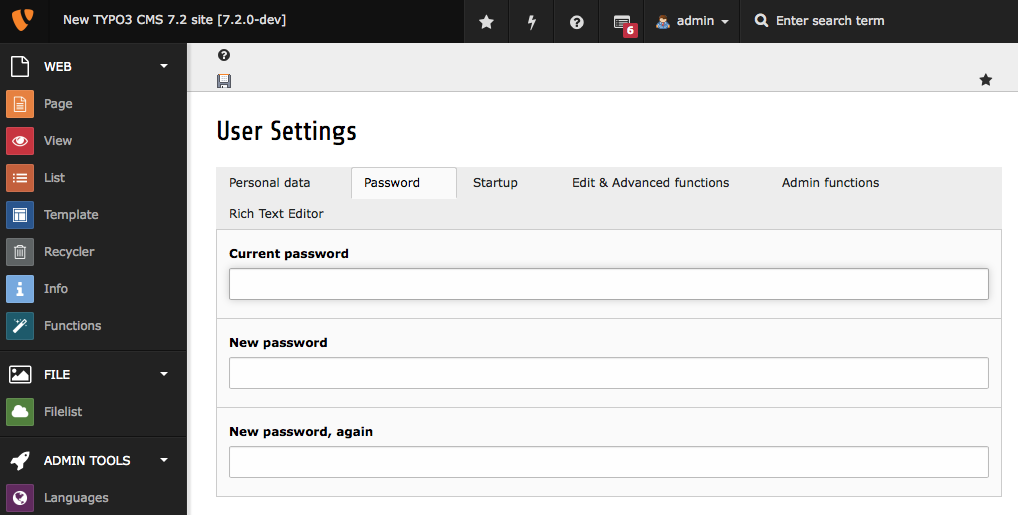
\includegraphics[width=0.7\linewidth]{BackendUserInterface/Password.png}
	\end{figure}

\end{frame}

% ------------------------------------------------------------------------------
% LTXE-SLIDE-START
% LTXE-SLIDE-UID:		4479d9ca-dfa0e494-1054e1b9-b025d605
% LTXE-SLIDE-ORIGIN:	7725bce9-e606f055-bf2e7b4a-e870fe2a English
% LTXE-SLIDE-TITLE:		Add icon for "Show Content From Page"
% LTXE-SLIDE-REFERENCE:	commit f8aa3eea9aed97a901ef0c3e7c650e1218839596
% ------------------------------------------------------------------------------
\begin{frame}[fragile]
	\frametitle{Interfaz de Usuario de Backend}
	\framesubtitle{Icono de página para "Mostrar Contenido de la Página"}

	Un nuevo icono de página en el árbol de navegación indica que una página
	muestra contenido de otra página:

	\begin{figure}
		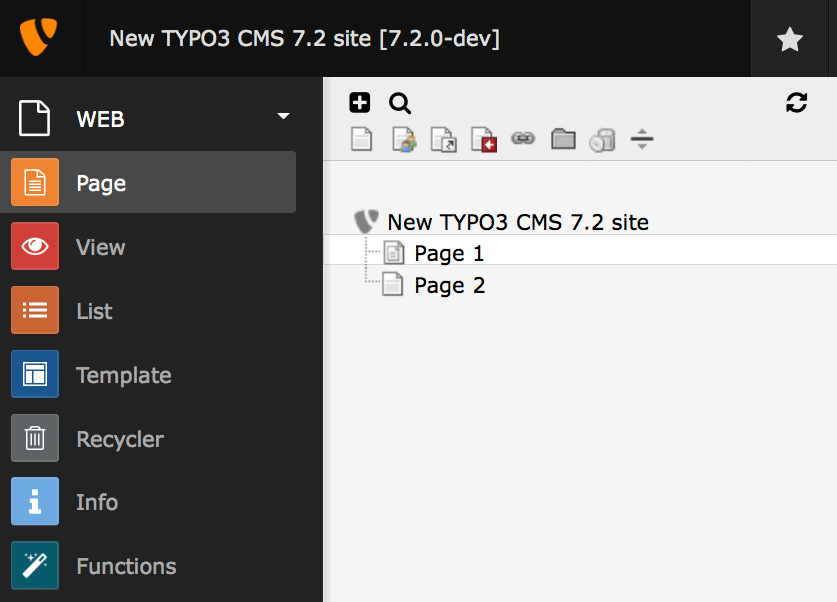
\includegraphics[width=0.45\linewidth]{BackendUserInterface/ShowContent.png}
	\end{figure}

\end{frame}

% ------------------------------------------------------------------------------
% LTXE-SLIDE-START
% LTXE-SLIDE-UID:		0e1370b3-e1f47fb9-a34bd18f-7ed59a4a
% LTXE-SLIDE-ORIGIN:	5ac2de45-9be12bf9-1c326192-602839fb English
% LTXE-SLIDE-TITLE:		Extension Manager: Choose version for update
% LTXE-SLIDE-REFERENCE:	commit a26396a4530b530744ec8b36c5fb5606789a6739
% ------------------------------------------------------------------------------
\begin{frame}[fragile]
	\frametitle{Interfaz de Usuario de Backend}
	\framesubtitle{Actualizaciones de Extensiones}

	Al actualizar una extensión, es posible elegir la versión destino:

	\begin{figure}
		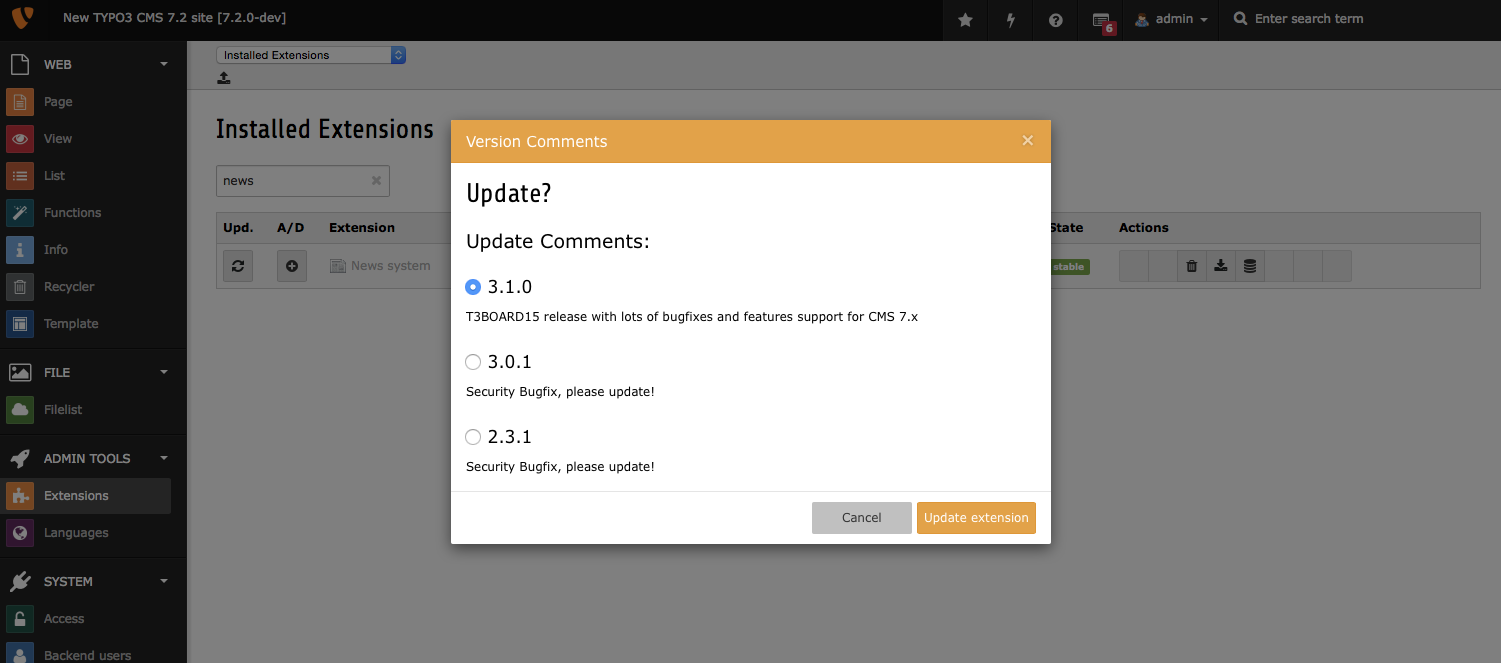
\includegraphics[width=0.75\linewidth]{BackendUserInterface/Update.png}
	\end{figure}

\end{frame}

% ------------------------------------------------------------------------------
% LTXE-SLIDE-START
% LTXE-SLIDE-UID:		432d69e9-0d4b4072-18ff14b4-c3b98543
% LTXE-SLIDE-ORIGIN:	f6be31f7-155d676c-0e551545-3fc89e89 English
% LTXE-SLIDE-TITLE:		Add scheduler task to remove deleted records
% LTXE-SLIDE-REFERENCE:	Feature-32651-AddSchedulerTaskToRemoveDeletedRecords.rst
% ------------------------------------------------------------------------------
\begin{frame}[fragile]
	\frametitle{Interfaz de Usuario de Backend}
	\framesubtitle{Tarea Recycler}

	Una nueva tarea del planificador para la extensión de sistema \texttt{recycler}
	borra los registros eliminados de las tablas de contenido en la base de
	datos. La edad máxima y las tablas afectadas son configurables en los ajustes
	de la tarea. Esto se puede también aplicar a los archivos.

	\begin{figure}
		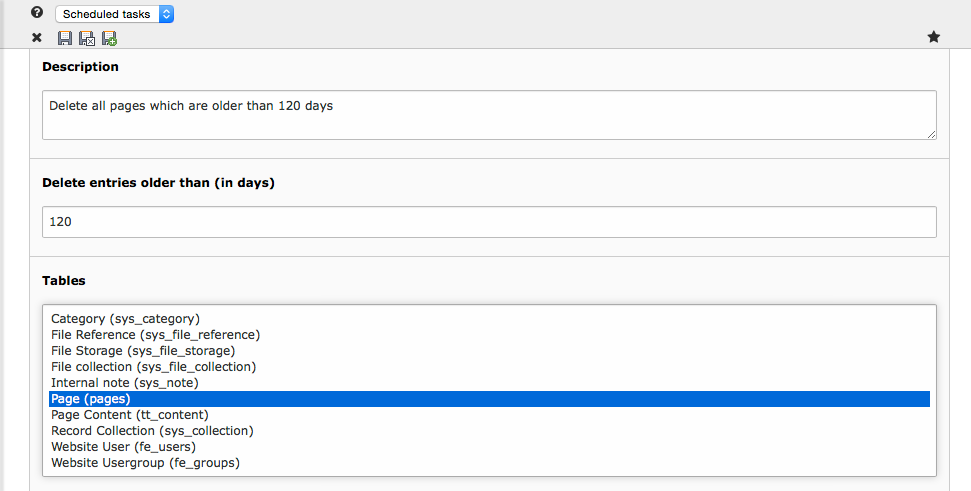
\includegraphics[width=0.68\linewidth]{BackendUserInterface/RecyclerTask.png}
	\end{figure}

\end{frame}

% ------------------------------------------------------------------------------
